
\subsection{Différences de résultat}
En comparant les images ci-dessus, nous pouvons observer quelques différences entre la méthode de Fourier et les deux autres. En effet, la méthode des différences finies ne travaille que sur une partie de l'image, celle qui va être collée, afin de l'adapter au mieux à l'image de fond. Le reste de l'image n'est pas modifié et on retrouve exactement l'image initiale T en dehors du domaine.(tout comme l'algorithme de Douglas). \\
La méthode de Fourier elle, modifie toute l'image, elle n'adapte pas seulement la partie à coller, mais c'est toute l'image qui est modifiée. Fourier effectue un "mélange" des deux images. \\
Plus la précision de l'algorithme de Douglas augmente, plus le résultat obtenu avec celui-ci est proche de celui obtenu avec les différences finies.
\subsection{Différence de temps}
La méthode des différences finies fait intervenir une inversion matricielle, qui si elle est grande, augmentera significativement le temps de calcul de l'algorithme. Cette méthode consiste en la résolution d'un système plus ou moins grand, qui peut parfois prendre du temps. \\
Sur de grandes sélections, la méthode de Fourier, semble plus rapide, il est facile de calculer le gradient de l'image, et la fft ("fast fourier transform") est plus rapide. Sur de grandes sélections c'est donc cette méthode qui serait à privilégier.\\
L'image ci-dessous présente une comparaison des temps de calcul de Fourier et des différences finies en fonction de la sélection. L'image choisie est de taille $(800 \times 450 \times 3)$ :
\begin{figure}[H]
\centering
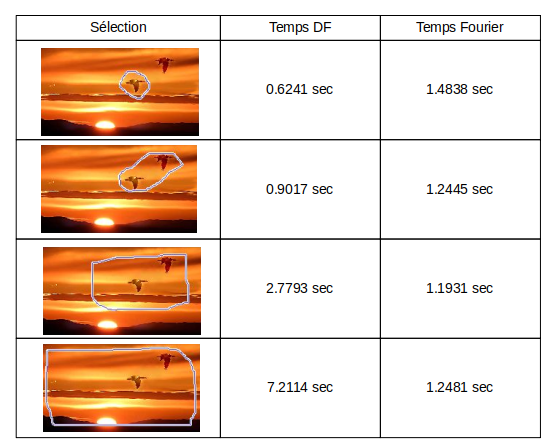
\includegraphics[scale=0.4]{Images/comparaisonFD.png}
\caption{Comparaison en fonction de la sélection}
\end{figure}
La méthode de Douglas, est beaucoup plus lente, à cause du coût de l'opérateur proximal de $f$, et du nombre d'itérations répétées.  
